% Options for packages loaded elsewhere
\PassOptionsToPackage{unicode}{hyperref}
\PassOptionsToPackage{hyphens}{url}
\documentclass[
  american,
  12pt,
  letterpaper,
]{article}
\usepackage{xcolor}
\usepackage{amsmath,amssymb}
\setcounter{secnumdepth}{5}
\usepackage{iftex}
\ifPDFTeX
  \usepackage[T1]{fontenc}
  \usepackage[utf8]{inputenc}
  \usepackage{textcomp} % provide euro and other symbols
\else % if luatex or xetex
  \usepackage{unicode-math} % this also loads fontspec
  \defaultfontfeatures{Scale=MatchLowercase}
  \defaultfontfeatures[\rmfamily]{Ligatures=TeX,Scale=1}
\fi
\usepackage{lmodern}
\ifPDFTeX\else
  % xetex/luatex font selection
\fi
% Use upquote if available, for straight quotes in verbatim environments
\IfFileExists{upquote.sty}{\usepackage{upquote}}{}
\IfFileExists{microtype.sty}{% use microtype if available
  \usepackage[]{microtype}
  \UseMicrotypeSet[protrusion]{basicmath} % disable protrusion for tt fonts
}{}
\makeatletter
\@ifundefined{KOMAClassName}{% if non-KOMA class
  \IfFileExists{parskip.sty}{%
    \usepackage{parskip}
  }{% else
    \setlength{\parindent}{0pt}
    \setlength{\parskip}{6pt plus 2pt minus 1pt}}
}{% if KOMA class
  \KOMAoptions{parskip=half}}
\makeatother
\usepackage{graphicx}
\makeatletter
\newsavebox\pandoc@box
\newcommand*\pandocbounded[1]{% scales image to fit in text height/width
  \sbox\pandoc@box{#1}%
  \Gscale@div\@tempa{\textheight}{\dimexpr\ht\pandoc@box+\dp\pandoc@box\relax}%
  \Gscale@div\@tempb{\linewidth}{\wd\pandoc@box}%
  \ifdim\@tempb\p@<\@tempa\p@\let\@tempa\@tempb\fi% select the smaller of both
  \ifdim\@tempa\p@<\p@\scalebox{\@tempa}{\usebox\pandoc@box}%
  \else\usebox{\pandoc@box}%
  \fi%
}
% Set default figure placement to htbp
\def\fps@figure{htbp}
\makeatother
\ifLuaTeX
\usepackage[bidi=basic,shorthands=off]{babel}
\else
\usepackage[bidi=default,shorthands=off]{babel}
\fi
\ifLuaTeX
  \usepackage{selnolig} % disable illegal ligatures
\fi
\setlength{\emergencystretch}{3em} % prevent overfull lines
\providecommand{\tightlist}{%
  \setlength{\itemsep}{0pt}\setlength{\parskip}{0pt}}
\usepackage[margin=1.24in]{geometry}
\usepackage{setspace}
\usepackage{graphicx}
\usepackage{xcolor}
\usepackage{helvet}
\usepackage{titlesec}
\usepackage{fancyhdr}
\usepackage{booktabs}
\usepackage{longtable}
\usepackage{array}
\usepackage{hyperref}
\definecolor{BookGold}{HTML}{FFD166}
\definecolor{BookBone}{HTML}{F6E8C8}
\definecolor{BookEmber}{HTML}{FF5E3A}
\definecolor{BookInk}{HTML}{12171F}
\renewcommand{\familydefault}{\rmdefault}
\setstretch{1.31}
\setlength{\parindent}{0pt}
\setlength{\parskip}{1.05em}
\raggedbottom
\titleformat{\section}{\normalfont\Large\bfseries\sffamily\color{BookEmber}}{\thesection}{0.7em}{}
\titleformat{\subsection}{\normalfont\large\bfseries\sffamily\color{BookGold}}{\thesubsection}{0.7em}{}
\hypersetup{
  colorlinks=true,
  linkcolor=BookEmber,
  urlcolor=BookEmber,
  citecolor=BookEmber
}
\pagestyle{fancy}
\fancyhf{}
\fancyhead[L]{\sffamily\small\textcolor{BookInk}{Children of the Feed}}
\fancyhead[R]{\sffamily\small\textcolor{BookInk}{\nouppercase{\leftmark}}}
\fancyfoot[C]{\sffamily\small\thepage}
\setlength{\headheight}{14pt}
\usepackage{bookmark}
\IfFileExists{xurl.sty}{\usepackage{xurl}}{} % add URL line breaks if available
\urlstyle{same}
% fallback for those not using the hyperref driver hyperxmp:
\makeatletter
\@ifundefined{xmpquote}{\newcommand{\xmpquote}[1]{#1}}{}
\makeatother
\hypersetup{
  pdftitle={The Three Reforms},
  pdflang={en-US},
  hidelinks,
  pdfcreator={LaTeX via pandoc}}

\title{The Three Reforms}
\author{}
\date{}

\begin{document}
\maketitle

\section{The Three Reforms}\label{the-three-reforms}

\subsection{Deck}\label{deck}

The response is no longer a mood. It is a program.

\begin{figure}
\centering
\pandocbounded{
\includegraphics[keepaspectratio,alt={Chapter 10 cover}]{../assets/generated/covers/10_the-three-reforms_cover.png}}
\caption{Chapter 10 cover}
\end{figure}

\subsection{Opening}\label{opening}

This book does not end with a self-care checklist and a request for
nicer billionaires.

It does not end with ``maybe unplug more.''

It does not end with ``hopefully the market figures it out.''

And it definitely does not end with the exhausted fantasy that if users
just become a little more disciplined, the architecture itself will
somehow stop being extractive.

No.

The problem is structural.

So the answer has to become structural too.

If the feed became territory, if the archive became private capability,
and if access to advanced intelligence is being consolidated through
state-adjacent corporate power, then a serious response has to move at
the level of law, ownership, and public obligation.

That is why this book closes with three reforms, not thirty vibes.

There is a reason the ending has to sound firmer than the opening. By
this point the reader has already walked through the harvest, the social
damage, the acceleration, the enclosure, the layoffs, the access
hierarchy, and the legitimacy theater. If the book ended with ``it's
complicated,'' that would not be nuance. That would be surrender in
expensive prose.

\subsection{Main Narrative}\label{main-narrative}

\subsubsection{Refactor Section 230}\label{refactor-section-230}

The first reform is to refactor Section 230 around reality rather than
nostalgia.

The old legal imagination behind platform immunity was built for an era
when the internet could still be pictured as a host environment rather
than a behavioral command architecture. That imagination is obsolete. It
does not describe what sovereign-scale platforms actually do.

These systems do not merely store speech. They rank it, amplify it,
suppress it, route it, recommend it, monetize it, target it, and build
predictive systems out of its aftermath. They shape what rises, what
disappears, what becomes desirable, what becomes punishing, what is
rewarded, and what is rendered socially invisible.

That is not neutral carriage.

That is governance by design.

If a system can tune visibility for billions, it is not a passive
intermediary in any meaningful moral sense. It is infrastructure with
editorial, psychological, and civic consequences at scale. A platform
this powerful can no longer receive the same liability logic as if it
were a dumb wall covered in stranger graffiti.

What should replace that fiction? Responsibility keyed to reach,
amplification power, monetization structure, targeting architecture,
moderation design, and systemic harm. Not perfection. Not impossible
prior review of all human speech. But real duties proportional to power.

This is especially important for the generations this book is written
to. Gen Z and millennials did not mainly encounter these systems as
abstract policy entities. They encountered them as developmental
environments. Systems that shaped beauty, status, sexual signaling,
moral outrage, belonging, loneliness, and attention collapse. The law
cannot keep acting as if all of that was random user behavior floating
on top of neutral plumbing.

We are past that stage.

The platform is not just where harm happens.

The platform is often part of how harm is formatted, intensified, and
monetized.

What this means in ordinary language is simple: if a company designs the
weather, it cannot keep pretending it merely hosts the rain. Once a
system ranks desire, outrage, beauty, panic, belonging, and humiliation
at population scale, it becomes part of the causal machinery of the
social world. That does not require impossible liability for every
utterance. It requires ending the childish fiction that sovereign-scale
behavioral infrastructures are just neutral bulletin boards with better
branding.

\begin{figure}
\centering
\pandocbounded{
\includegraphics[keepaspectratio,alt={Chapter 10 reform illustration}]{../assets/generated/illustrations/10_the-three-reforms_scene_a.png}}
\caption{Chapter 10 reform illustration}
\end{figure}

\subsubsection{AI Weights as Patrimony of
Humanity}\label{ai-weights-as-patrimony-of-humanity}

The second reform is to treat frontier AI weights trained on humanity's
collective expression as a patrimony question, not merely a
private-property question.

This is the intellectual heart of the whole project.

If the systems now being sold as frontier intelligence are built from
human civilization in compressed form, then it is morally and
politically absurd to treat them as if they were ordinary assets
generated in a vacuum by whoever reached the compute cluster first. Not
because current law has already settled the matter. It has not. But
because the social reality already outruns the inherited categories.

A frontier weight is not a human mind.

It is not a literal copy of civilization.

It is not a soul in a server rack.

But it is also not detached from the public archive that made it
possible.

That archive includes language, culture, art, code, expertise, memory,
style, pedagogy, and labor created across societies, classes, and
generations under wildly unequal conditions of consent and compensation.
Once that collectively generated world becomes private machine power,
the burden should shift. Firms should have to justify enclosure, not the
public justify why it deserves a stake in what was built from its
residue.

That is what patrimony means here. A framework in which frontier
capability triggers public-trust reasoning, anti-monopoly limits,
democratic oversight, transparency obligations, and a presumption
against total private enclosure of intelligence built from collective
life.

The end state argued for in this book is not naive chaos.

It is not ``release everything and hope for the best.''

It is not pretending there are zero safety concerns.

It is something more demanding: move the center of gravity away from
permanent private scarcity and toward broad public-interest
availability, utility-like obligations, and governance structures that
acknowledge the collective origin of the capability.

Put differently:

If humanity helped build the field, humanity should not be treated as a
mere customer standing outside the fence.

And that is where this project parts ways with the timid version of
reform. Too much public debate still treats the weights fight like a
niche copyright argument for specialists. It is bigger than that. It is
a civilizational ownership argument. Either intelligence built from
collective human residue remains permanently enclosed by whoever
captured the best legal and compute position first, or we admit that a
capability generated from humanity at scale carries public-trust
implications by default.

\subsubsection{Limit Government Capture by AI
Companies}\label{limit-government-capture-by-ai-companies}

The third reform is to limit government capture by AI companies and,
just as importantly, limit corporate capture of public intelligence
infrastructure.

This one matters because private concentration gets even more dangerous
once it fuses with public power under low-visibility conditions. If a
small number of frontier firms sit inside procurement channels, defense
pathways, national-security coordination, public funding streams,
export-control privilege, or strategic state access, then their
obligations should increase dramatically.

No more soft-focus language about partnership as if partnership itself
were automatically virtuous.

No more pretending that public dependence on private intelligence
vendors is just another procurement detail.

No more shrugging at revolving doors, lobbying intensity, opaque
model-risk practices, or selective disclosure because everyone is too
mesmerized by the product layer.

If public institutions are going to rely on frontier AI systems, then
the public gets a right to more than glossy marketing and elite
reassurance.

At minimum, that means:

\begin{itemize}
\tightlist
\item
  procurement visibility
\item
  conflict-of-interest disclosure
\item
  lobbying disclosure
\item
  public reporting on material government interaction
\item
  independent audit structures
\item
  model-risk disclosure
\item
  transparency around public support and strategic privilege
\item
  limits on exclusive private benefit where public backing materially
  strengthens the underlying infrastructure
\end{itemize}

This is not anti-state coordination. States will obviously interact with
major AI systems. The point is not to ban contact. The point is to stop
treating opaque entanglement as normal. A firm that receives public
support, public privilege, or national-security intimacy while
controlling a layer of future intelligence infrastructure should be
judged less like a charismatic startup and more like a public-risk actor
with heightened obligations.

That is the anti-capture doctrine in plain language:

the closer a private firm gets to public intelligence infrastructure,
the less acceptable secrecy, unilateral enclosure, and unaccountable
privilege become.

\begin{figure}
\centering
\pandocbounded{
\includegraphics[keepaspectratio,alt={Chapter 10 reform doctrine infographic}]{../assets/generated/infographics/10_the-three-reforms_infographic_b.png}}
\caption{Chapter 10 reform doctrine infographic}
\end{figure}

\begin{figure}
\centering
\pandocbounded{
\includegraphics[keepaspectratio,alt={Chapter 10 reform illustration B}]{../assets/generated/illustrations/10_the-three-reforms_scene_b.png}}
\caption{Chapter 10 reform illustration B}
\end{figure}

\begin{figure}
\centering
\pandocbounded{
\includegraphics[keepaspectratio,alt={Chapter 10 reform illustration C}]{../assets/generated/illustrations/10_the-three-reforms_scene_c.png}}
\caption{Chapter 10 reform illustration C}
\end{figure}

Everything else readers may want to do still matters. Digital hygiene
matters. Cognitive recovery matters. Labor organization matters.
Competition policy matters. Open public infrastructure matters. Youth
education matters. Cultural criticism matters. Refusing total dependence
matters.

But those are not alternatives to the three reforms.

They are what make the reforms livable.

They are implementation arms, not substitutes.

That distinction is important because a lot of public conversation gets
trapped at the lifestyle layer. Should we use the tools less? Should
parents monitor more? Should workers reskill? Should artists adapt?
Sure, some of that has a place. But if the architecture of extraction,
enclosure, and capture remains intact, lifestyle adaptation becomes
unpaid maintenance of a system that keeps deepening the harm.

\begin{figure}
\centering
\pandocbounded{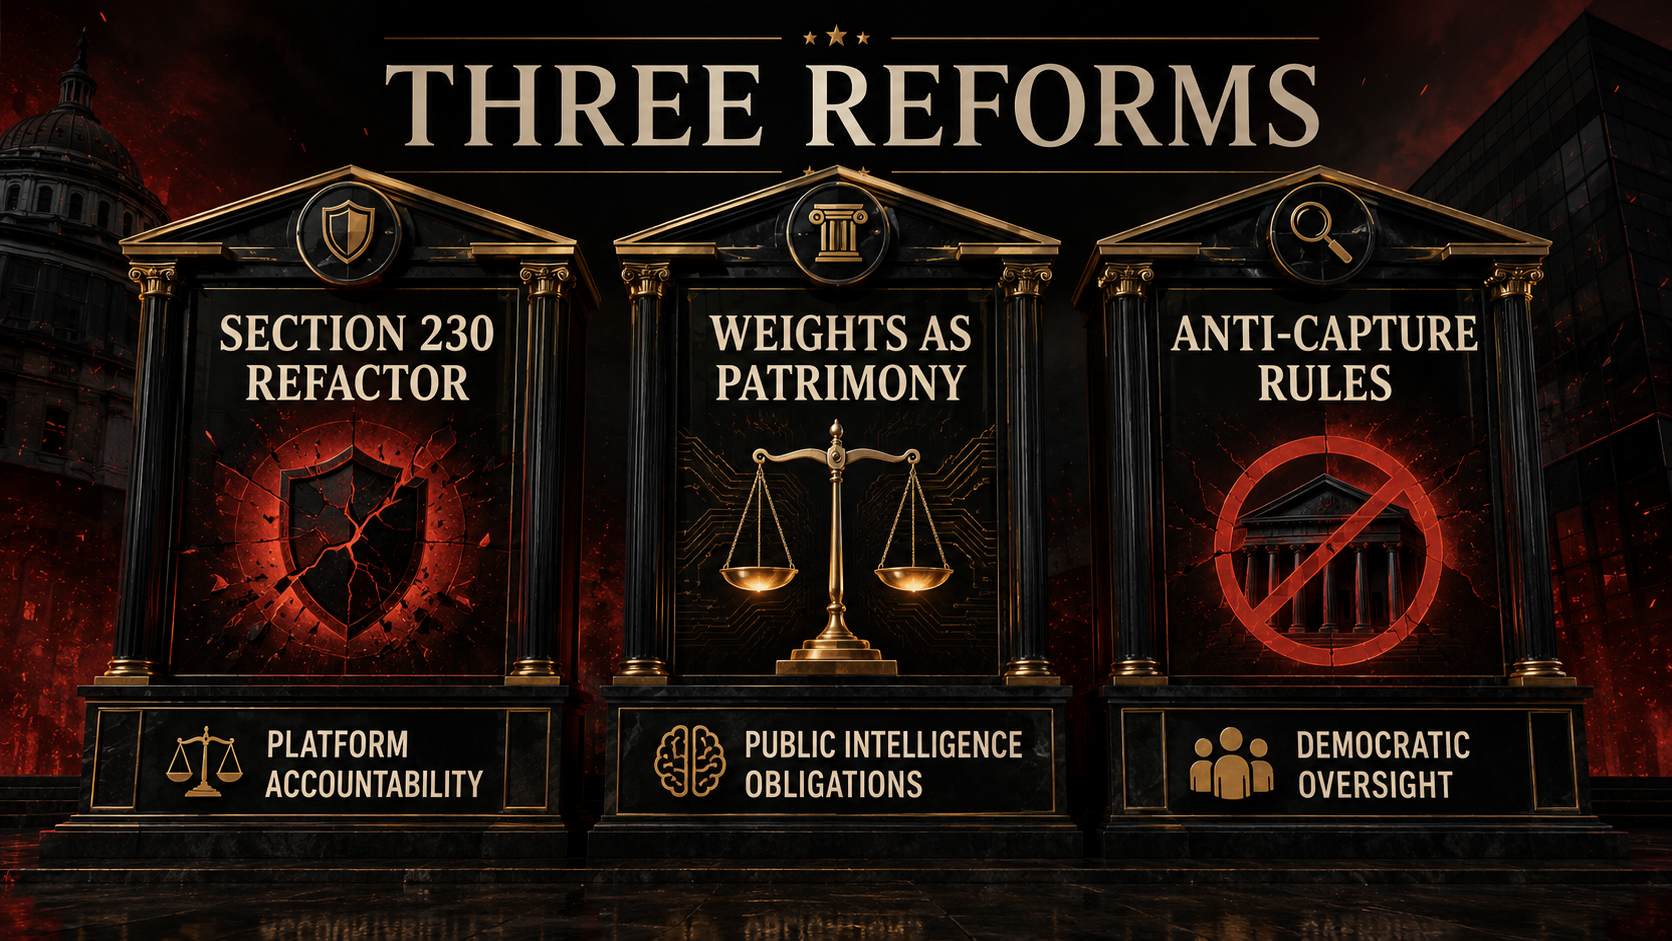
\includegraphics[keepaspectratio,alt={Chapter 10 reform infographic}]{../assets/generated/infographics/10_the-three-reforms_infographic_a.png}}
\caption{Chapter 10 reform infographic}
\end{figure}

The point of ending with reforms is not to pretend politics is easy.

It is to refuse the fake maturity that says diagnosis without doctrine
is enough.

It isn't.

A generation needs more than critique.

It needs naming.

Then structure.

Then terms of refusal.

Then terms of reconstruction.

That is the real emotional promise this book is trying to keep with the
reader. You are not crazy for feeling that something broke. You are not
weak because the feed rewired you. You are not obsolete because a model
can imitate pieces of your labor. You are not overreacting because the
state-company relationship around frontier AI feels off. You are living
inside a system that industrialized dependency and is now trying to
rename the result as destiny.

Destiny is the word power uses when it wants obedience without debate.

This book rejects that word.

The future is not something these firms get to inherit by default
because they were first to turn our residue into machine power.

The future is still a governance fight.

And if we are serious, it starts here:

Refactor Section 230.

Treat AI weights as a patrimony of humanity question.

Limit government capture by AI companies.

Everything else depends on whether those three moves become thinkable at
scale.

\subsection{Research Basis}\label{research-basis}

This chapter adapts the documentary argument developed in the research
paper
\href{../../papers/html/10_three-reform-program_paper.html}{\textbf{Chapter
10: What To Do}}. The PDF version is
\href{../../papers/pdf/10_three-reform-program_paper/10_three-reform-program_paper.pdf}{here}.
That paper states the three-reform program directly and grounds it in
the documented upstream record on platform design, training conflict,
access control, and institutional capture.

\subsection{Next}\label{next}

The literary book ends here, but the work it argues for begins outside
the page: in law, in labor, in public language, in technical governance,
and in the refusal to keep calling extraction inevitable just because it
learned how to speak back.

\end{document}
